
\chapter{Comparison to MD simulation\label{chpt:ions}}

In the last chapter, we have proven that \acs{MDFT} is capable to
correctly predict solvation properties of LJ centers, single ions
and linear solutes compared to \acs{IET}. In this section, we will
compare them to \acs{MD} and experimental results. All the solutes
are optimized with the fast \texttt{\textbf{convolution\_standard}}
algorithm, with implicitly $L=24$ $\textrm{Å}$, $\mathrm{nfft}=72$,
$m_{\max}=n_{\max}$ unless otherwise specified. Comparison to dipole
method is also involved in, as we should justify that the increase
of computing cost is has the capability to produce better results. 

\section{LJ centers}

The \acs{RDF} of rare gases calculated in \ref{tab:Free-energy-rare-gas}
is compared to \acs{MD} in figure \ref{fig:rare-gazz} using $n_{\max}=3$
to 5. The structures of different $n_{\max}$ is almost identical.
Comparing to \acs{MD}, it looks like there is no improvement compared
to the dipole method in ref \citep{Zhao_2011} \textcolor{red}{or
to calculation involving $c_{00}^{000}$ only.} This kind of disagreement
in curve shape is regarded as a known default of \acs{HNC} approximation.

\begin{figure}[h]
\begin{centering}
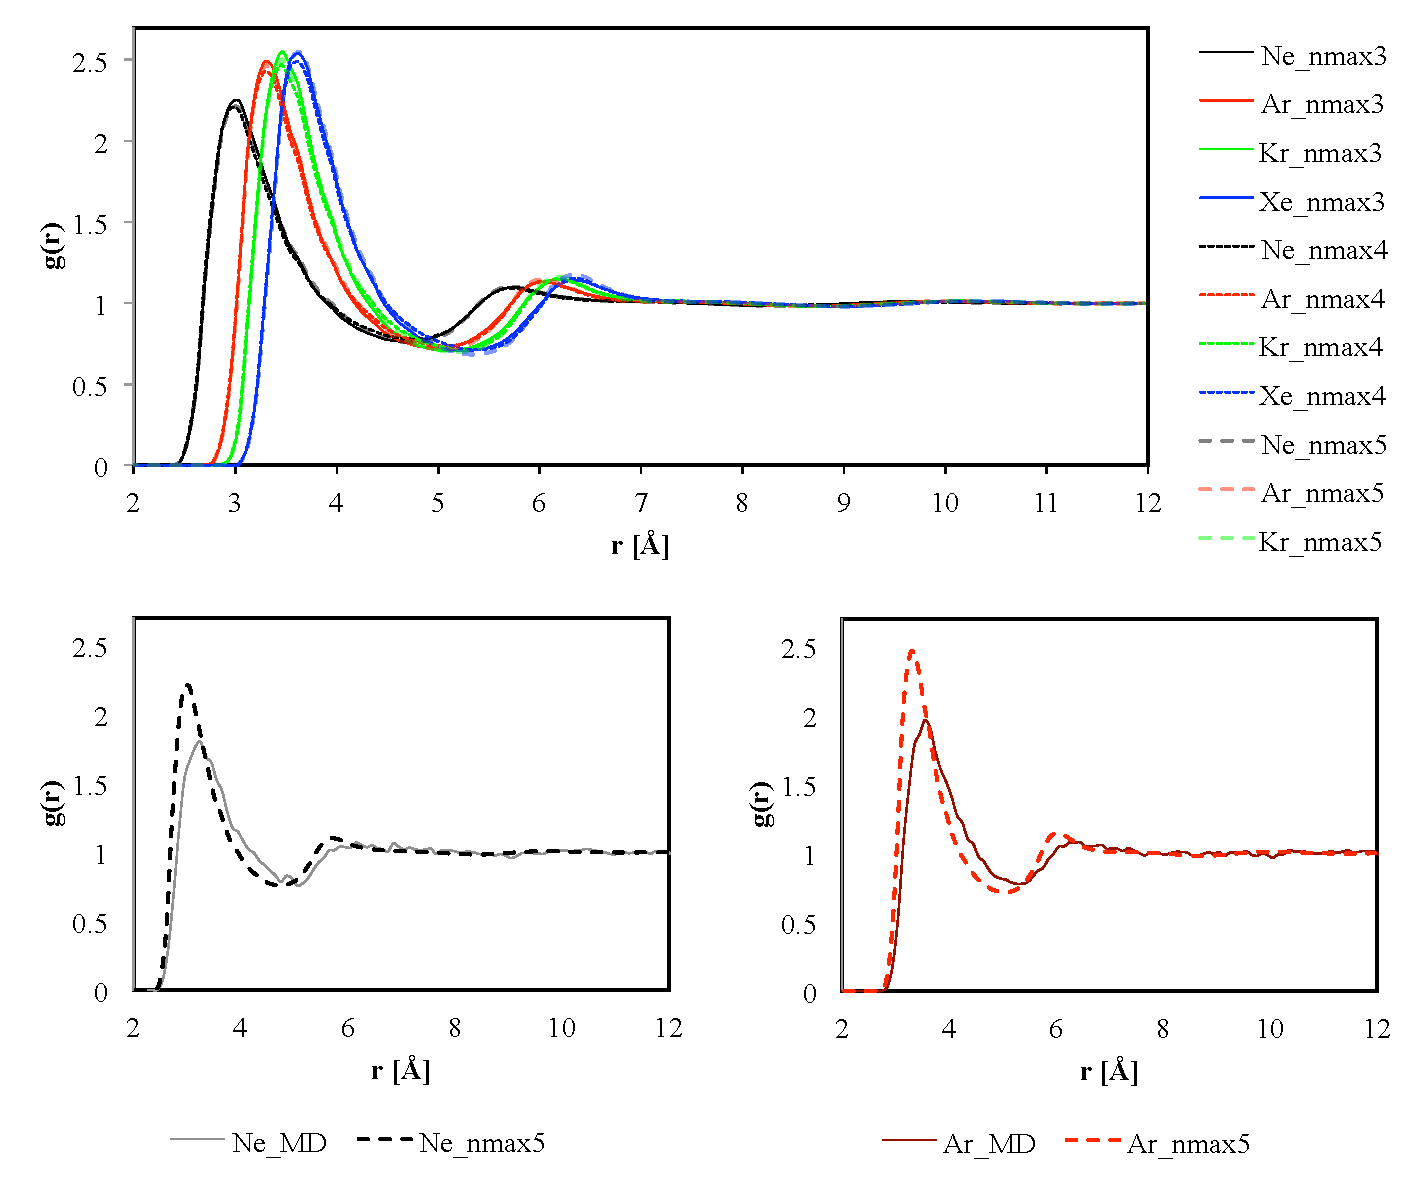
\includegraphics[width=0.9\columnwidth]{_figure/results/rare_gaz}
\par\end{centering}
\caption{\acs{RDF} of rare gazes compared to \acs{MD} result\label{fig:rare-gazz}}
\end{figure}


\section{Charged $\mathrm{CH_{4}}$ series}

The comparison of \acs{RDF} with \acs{MD} results for charged $\mathrm{CH_{4}}$
series are shown in figure \ref{fig:Comparison-to-MD}. We can see
that for positive charges, the complete $n_{\max}=5$ gives much better
results compared to dipole method, which is almost well agreed with
\acs{MD} results. For negative charges, $n_{\max}=5$ gives nearly
the same result as dipole method, while the \acs{MD} results are
more smooth, but the first peak of the \acs{MDFT} results seems to
be in good position. We can conclude that the complete \acs{DCF}
gives a large improvement for positive charged ions.

\begin{figure}[h]
\begin{centering}
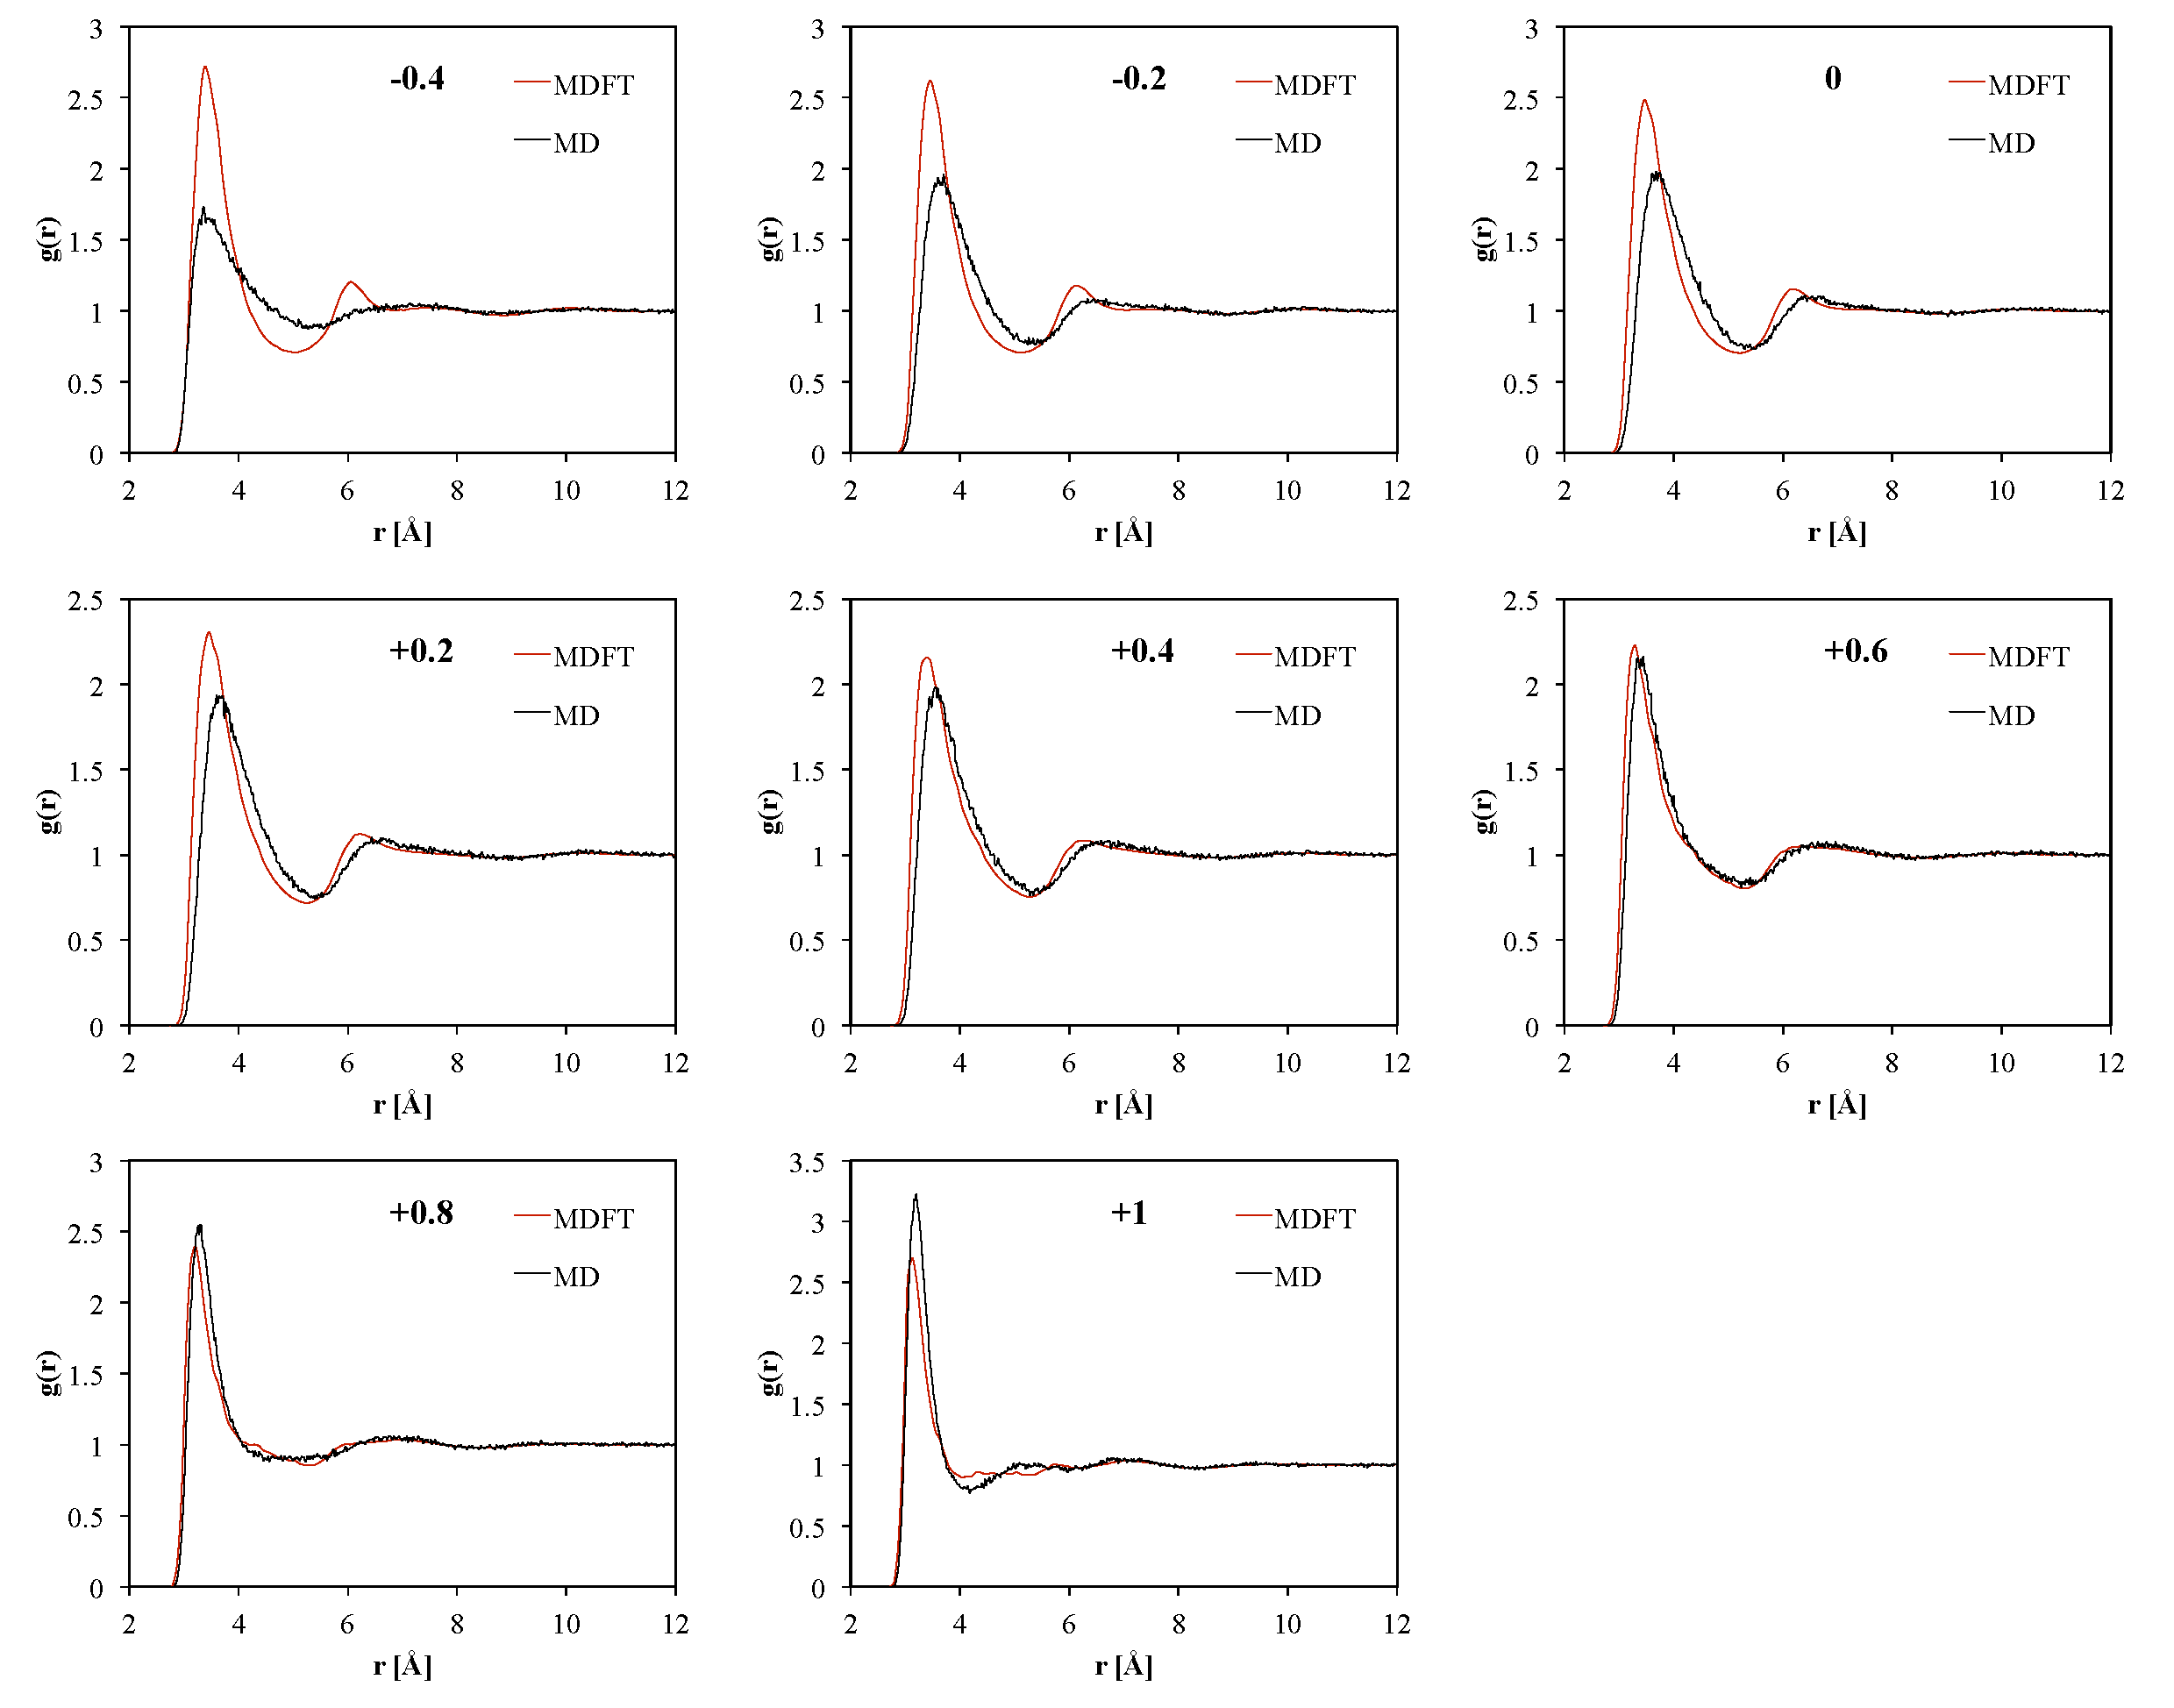
\includegraphics[width=1\columnwidth]{_figure/results/ch4_md}
\par\end{centering}
\caption{\acs{RDF} of charged $\mathrm{CH_{4}}$ series compared to \acs{MD}
result\label{fig:Comparison-to-MD}}
\end{figure}


\section{Solvation free energy of single ions}

\marginpar{We consider that for a macroscopic system, when the number of particles
$N\rightarrow\infty$, the Gibbs and Helmholtz free energy are almost
the same. \citep{ensemble_thermo}}From above we can see the \acs{RDF} for positive ions are in well
agreement with \acs{MD} results. However, the energy is more difficult
to compare, as there are several conventions of single ions, depending
on for example box length and charge; and the free energy depends
largely on the input LJ parameters of the ions, which is independent
to the method.

Table \ref{tab:single-ions} gives some experimental and \acs{MD}
simulation result of solvation free energy and first maximum of \acs{RDF}
for alkali and halide ions. We can see that the data itself varies
a lot. Nevertheless, the LJ parameters of ions from literatures can
also have thousand times of difference. Therefore, we chose a series
of force field parameters for halide anions and alkali cations from
ref \citep{horinek_rational_2009} based on SPC/E water as shown also
in table \ref{tab:single-ions}. 

\begin{table}[h]
\begin{centering}
\begin{tabular*}{1\linewidth}{@{\extracolsep{\fill}}ccccccccc}
\toprule 
\addlinespace[-0.17em]
\tableheadline{{\footnotesize{}Ion}} & {\scriptsize{}$-\Delta G_{\mathrm{solv}}^{\mathrm{exp}}$\textsuperscript{{\scriptsize{}(a)}}} & {\scriptsize{}$-\Delta F_{\mathrm{solv}}^{\mathrm{exp}}$\textsuperscript{{\scriptsize{}(b)}}} & {\scriptsize{}$-\Delta G_{\mathrm{solv}}^{\mathrm{exp}}$\textsuperscript{{\scriptsize{}(c)}}} & {\scriptsize{}$R_{1}$\textsuperscript{{\scriptsize{}(d)}}} & {\scriptsize{}$\sigma$ $[\textrm{Å}]$\textsuperscript{{\scriptsize{}(e)}}} & {\scriptsize{}$\epsilon$ {[}$\mathrm{kJ\cdot mol^{-1}}${]}\textsuperscript{{\scriptsize{}(e)}}} & {\scriptsize{}$-\Delta G_{\mathrm{solv}}^{\mathrm{MD}}$\textsuperscript{{\scriptsize{}(e)}}} & {\scriptsize{}$R_{1}^{\mathrm{MD}}$\textsuperscript{{\scriptsize{}(e)}}}\tabularnewline
\midrule 
\addlinespace[-0.33em]
{\scriptsize{}$\mathrm{F^{-}}$} & {\scriptsize{}465} & {\scriptsize{}374.5} & {\scriptsize{}428.8} & {\scriptsize{}2.08} & {\scriptsize{}3.30} & {\scriptsize{}0.55} & {\scriptsize{}-430} & {\scriptsize{}2.74}\tabularnewline
\addlinespace[-0.33em]
{\scriptsize{}$\mathrm{Cl^{-}}$} & {\scriptsize{}340} & {\scriptsize{}318.4} & {\scriptsize{}304.2} & {\scriptsize{}2.36} & {\scriptsize{}3.78} & {\scriptsize{}0.52} & {\scriptsize{}-306} & {\scriptsize{}3.23}\tabularnewline
\addlinespace[-0.33em]
{\scriptsize{}$\mathrm{Br^{-}}$} & {\scriptsize{}315} & {\scriptsize{}289.5} & {\scriptsize{}227.4} & {\scriptsize{}2.80} & {\scriptsize{}4.00} & {\scriptsize{}0.37} & {\scriptsize{}-279} & {\scriptsize{}3.35}\tabularnewline
\addlinespace[-0.33em]
{\scriptsize{}$\mathrm{I^{-}}$ } & {\scriptsize{}275} & {\scriptsize{}252.3} & {\scriptsize{}240.0} & {\scriptsize{}2.89} & {\scriptsize{}4.25} & {\scriptsize{}0.32} & {\scriptsize{}-241} & {\scriptsize{}3.55}\tabularnewline
\addlinespace[-0.33em]
{\scriptsize{}$\mathrm{Li^{+}}$ } & {\scriptsize{}475} & {\scriptsize{}511.0} & {\scriptsize{}529.4} & {\scriptsize{}3.14} & {\scriptsize{}3.02} & {\scriptsize{}0.02} & {\scriptsize{}-520} & {\scriptsize{}1.91}\tabularnewline
\addlinespace[-0.33em]
{\scriptsize{}$\mathrm{Na^{+}}$ } & {\scriptsize{}365} & {\scriptsize{}411.5} & {\scriptsize{}423.8} & {\scriptsize{}2.63} & {\scriptsize{}3.49} & {\scriptsize{}0.02} & {\scriptsize{}-414} & {\scriptsize{}2.28}\tabularnewline
\addlinespace[-0.33em]
{\scriptsize{}$\mathrm{K^{+}}$ } & {\scriptsize{}295} & {\scriptsize{}337.2} & {\scriptsize{}352.0} & {\scriptsize{}3.19} & {\scriptsize{}3.85} & {\scriptsize{}0.02} & {\scriptsize{}-347} & {\scriptsize{}2.54}\tabularnewline
\addlinespace[-0.33em]
{\scriptsize{}$\mathrm{Rb^{+}}$ } & {\scriptsize{}275} & {\scriptsize{}316.0} & {\scriptsize{}329.3} & {\scriptsize{}3.37} & {\scriptsize{}no data} & {\scriptsize{}no data} & {\scriptsize{}no data} & {\scriptsize{}no data}\tabularnewline
\addlinespace[-0.33em]
{\scriptsize{}$\mathrm{Cs^{+}}$ } & {\scriptsize{}250} & {\scriptsize{}283.8} & {\scriptsize{}no data} & {\scriptsize{}3.65} & {\scriptsize{}4.17} & {\scriptsize{}0.02} & {\scriptsize{}-300} & {\scriptsize{}2.79}\tabularnewline
\bottomrule
\end{tabular*}
\par\end{centering}
\caption[Free energy and first maximum of ion-water oxygen \acs{RDF} for alkali
and halide ions from experimental and \acs{MD} simulation result]{Free energy in $[\mathrm{kJ\cdot mol^{-1}}]$ and first maximum of
ion-water oxygen radial distribution functions in $[\textrm{Å}]$
for alkali and halide ions from experimental and \acs{MD} simulation
result. (a). Ref \citep{MARCUS1994111}. (b). Ref \citep{Noyes_1962}.
(c) Ref \citep{tissandier_protons_1998}. (e) Ref \citep{horinek_rational_2009}
from \acs{MD} simulation. (d) Ref \citep{Marcus_1988}.\label{tab:single-ions}}

\vspace{0.5cm}

\begin{centering}
\begin{tabular*}{1\linewidth}{@{\extracolsep{\fill}}ccccccc}
\toprule 
\addlinespace[-0.17em]
\tableheadline{{\footnotesize{}Ion}} & {\scriptsize{}$\Delta G_{\mathrm{solv}}^{\mathrm{MD}}$} & {\scriptsize{}$\Delta\varOmega_{\mathrm{solv}}^{\mathrm{dipole}}$} & {\scriptsize{}$\Delta\varOmega_{\mathrm{solv}}^{\mathrm{nmax3}}$} & {\scriptsize{}$R_{1}^{\mathrm{MD}}$} & {\scriptsize{}$R_{1}^{\mathrm{dipole}}$} & {\scriptsize{}$R_{1}^{\mathrm{nmax3}}$}\tabularnewline
\midrule 
\addlinespace[-0.33em]
{\scriptsize{}$\mathrm{F^{-}}$ } & {\scriptsize{}-430} & {\scriptsize{}diverge} & {\scriptsize{}-368.47} & {\scriptsize{}2.74} & {\scriptsize{}-} & {\scriptsize{}2.71}\tabularnewline
\addlinespace[-0.33em]
{\scriptsize{}$\mathrm{Cl^{-}}$ } & {\scriptsize{}-306} & {\scriptsize{}diverge} & {\scriptsize{}-297.33} & {\scriptsize{}3.23} & {\scriptsize{}-} & {\scriptsize{}2.88}\tabularnewline
\addlinespace[-0.33em]
{\scriptsize{}$\mathrm{Br^{-}}$ } & {\scriptsize{}-279} & {\scriptsize{}diverge} & {\scriptsize{}-278.32} & {\scriptsize{}3.35} & {\scriptsize{}-} & {\scriptsize{}2.96}\tabularnewline
\addlinespace[-0.33em]
{\scriptsize{}$\mathrm{I^{-}}$ } & {\scriptsize{}-241} & {\scriptsize{}diverge} & {\scriptsize{}-253.42} & {\scriptsize{}3.55} & {\scriptsize{}-} & {\scriptsize{}3.12}\tabularnewline
\addlinespace[-0.33em]
{\scriptsize{}$\mathrm{Li^{+}}$ } & {\scriptsize{}-520} & {\scriptsize{}-707.73} & {\scriptsize{}-405.28} & {\scriptsize{}1.91} & {\scriptsize{}2.46} & {\scriptsize{}2.38}\tabularnewline
\addlinespace[-0.33em]
{\scriptsize{}$\mathrm{Na^{+}}$ } & {\scriptsize{}-414} & {\scriptsize{}-621.76} & {\scriptsize{}-366.00} & {\scriptsize{}2.28} & {\scriptsize{}2.54} & {\scriptsize{}2.54}\tabularnewline
\addlinespace[-0.33em]
{\scriptsize{}$\mathrm{K^{+}}$ } & {\scriptsize{}-347} & {\scriptsize{}-559.13} & {\scriptsize{}-338.37} & {\scriptsize{}2.54} & {\scriptsize{}2.63} & {\scriptsize{}2.70}\tabularnewline
\addlinespace[-0.33em]
{\scriptsize{}$\mathrm{Cs^{+}}$ } & {\scriptsize{}-300} & {\scriptsize{}-508.84} & {\scriptsize{}-316.06} & {\scriptsize{}2.79} & {\scriptsize{}2.88} & {\scriptsize{}2.88}\tabularnewline
\bottomrule
\end{tabular*}
\par\end{centering}
\caption{Free energies $[\mathrm{kJ\cdot mol^{-1}}]$ and first \acs{RDF}
maximum $[\textrm{Å}]$ of single ions from \acs{MDFT} results compared
to experimental results \label{tab:free-energy-single-ions}}
\end{table}

The results shows that the free energies given by \acs{MDFT} is not
perfect, but in the same order of magnitude as \acs{MD} results.
Results with \acs{DCF} of $n_{\max}=3$ works better than dipole
in energy, \textcolor{red}{but in terms of position of first solvation
maximum it gives the same result for positive ions, which is a little
different with \acs{MD} results. specially for $\mathrm{Li^{+}}$.
Which is not completely agreed with the previous $\mathrm{CH_{4}}$
results.}

\section{Small molecules}

Some solute structure are also generated to compare to \acs{MD},
shown in figure \ref{fig:Test-solutes-2} and table \ref{tab:Parameters-of-test-solutes-2}.

Figure \ref{fig:Site-O} gives the site-site \acs{RDF}s (solute site
to water O site) of $n_{\max}=4$, dipole and \acs{MD} results for
these test solutes. It is shown that in the most of cases, $n_{\max}=4$
gives better or the same results than dipole, apart from the cases
of water, specially SPC/E water. In methanol, the dipole method diverge.

In the purpose to show the the ability of \acs{MDFT} to show calculate
3D solute structure, due to the spherical coordinate system it adopt,
we show some 3D figure of solvent in figure \ref{fig:Volume-slice-of}
and \ref{fig:Iso-surface-of-solvent}. In figure \ref{fig:Iso-surface-of-solvent},
we can see the famous tetrahedral structure around the water molecule.
In SPC/E water, there is more density than expected on the north pole,
and this piece of density disappears with the extra charged added
on the TIP4P water.

\begin{figure}[H]
\begin{centering}
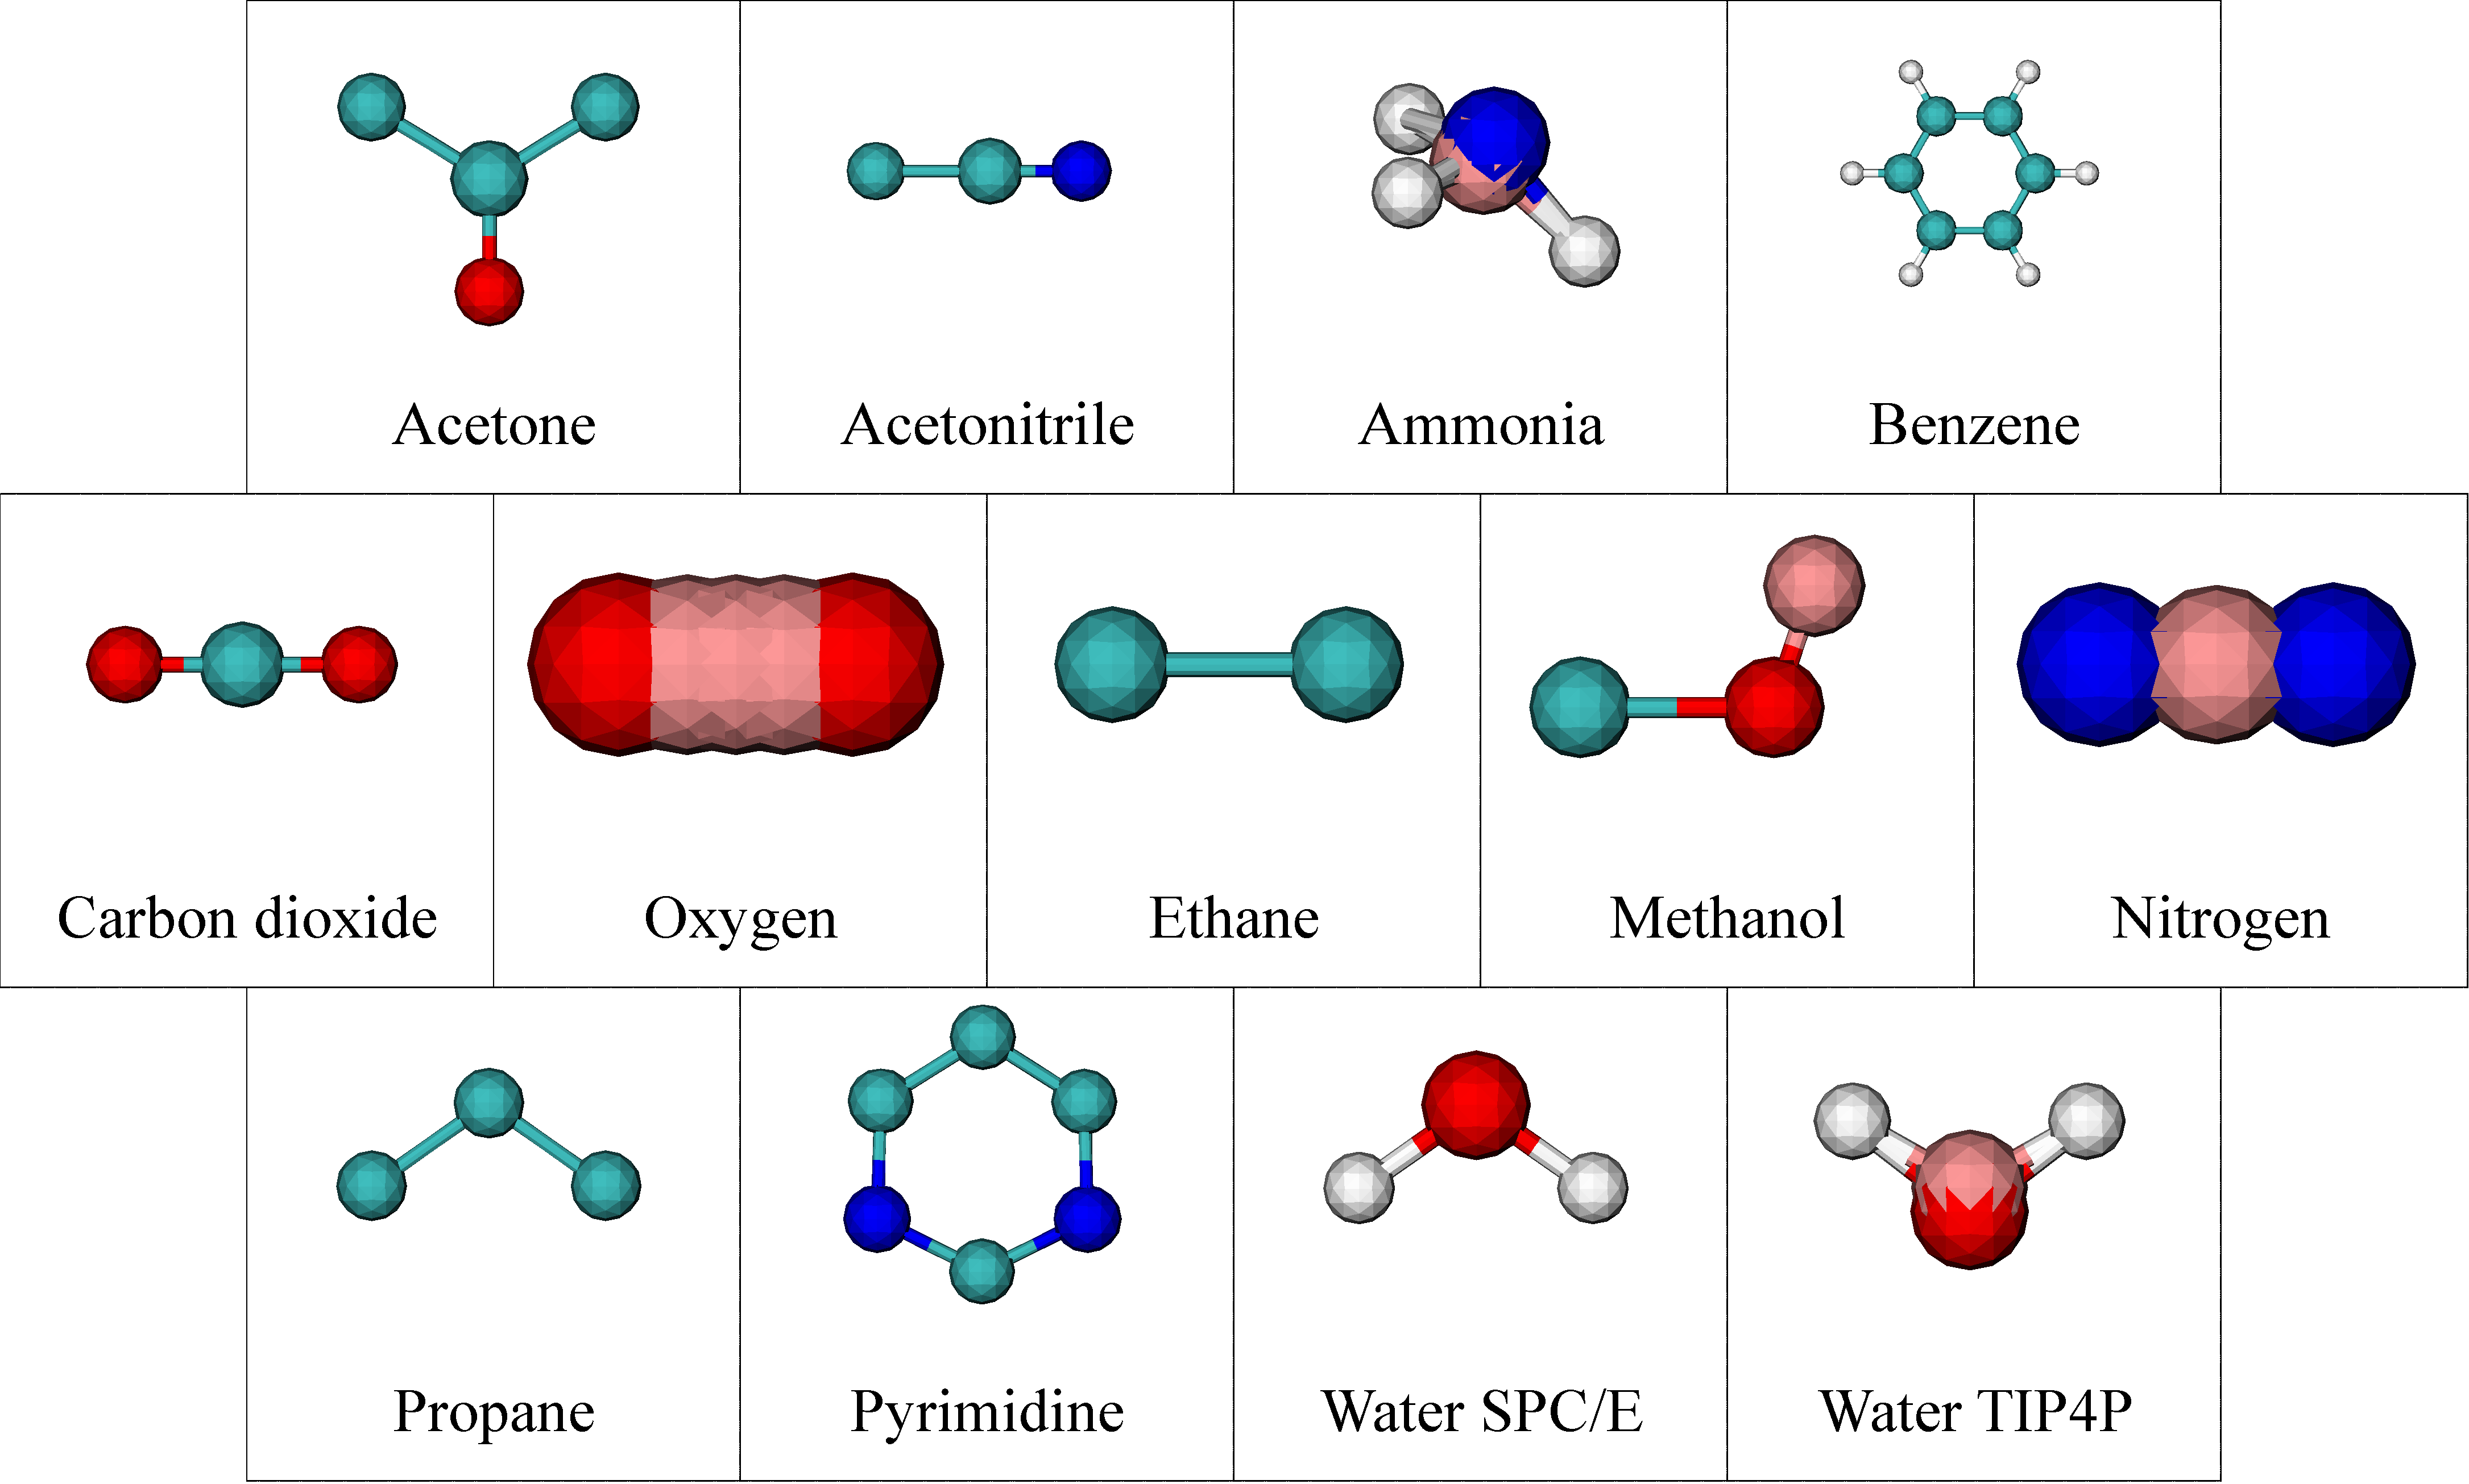
\includegraphics[width=1\columnwidth]{_figure/app_solute_var}
\par\end{centering}
\caption{Test solutes\label{fig:Test-solutes-2}}
\end{figure}

\begin{table}[H]
\begin{centering}
\begin{tabular*}{1\linewidth}{@{\extracolsep{\fill}}llrrrrrr}
\toprule 
\addlinespace[-0.17em]
\tableheadline{{\footnotesize{}Solute}} & \tableheadline{{\footnotesize{}Site}} & {\scriptsize{}$q$} & {\scriptsize{}$\sigma$ $[\textrm{Å}]$} & {\scriptsize{}$\epsilon$ {[}$\mathrm{kJ\cdot mol^{-1}}${]}} & {\scriptsize{}$x$ $[\textrm{Å}]$} & {\scriptsize{}$y$ $[\textrm{Å}]$} & {\scriptsize{}$z$ $[\textrm{Å}]$}\tabularnewline
\midrule 
\addlinespace[-0.33em]
{\scriptsize{}Acetone \citep{jorgensen_relative_1990}} & {\scriptsize{}CH\textsubscript{3}} & {\scriptsize{}0.062} & {\scriptsize{}3.91} & {\scriptsize{}0.6694} & {\scriptsize{}1.2810} & {\scriptsize{}0.7024} & {\scriptsize{}-0.0002}\tabularnewline
\addlinespace[-0.17em]
\addlinespace[-0.33em]
 & {\scriptsize{}C} & {\scriptsize{}0.300} & {\scriptsize{}3.75} & {\scriptsize{}0.4393} & {\scriptsize{}0.0101} & {\scriptsize{}-0.0872 } & {\scriptsize{}0.0106 }\tabularnewline
\addlinespace[-0.17em]
\addlinespace[-0.33em]
 & {\scriptsize{}O} & {\scriptsize{}-0.424} & {\scriptsize{}2.96} & {\scriptsize{}0.8796} & {\scriptsize{}0.0103} & {\scriptsize{}-1.3171 } & {\scriptsize{}-0.0102 }\tabularnewline
\addlinespace[-0.17em]
\addlinespace[-0.33em]
 & {\scriptsize{}CH\textsubscript{3}} & {\scriptsize{}0.062} & {\scriptsize{}3.91} & {\scriptsize{}0.6694} & {\scriptsize{}-1.2813} & {\scriptsize{}0.7019} & {\scriptsize{}-0.0002}\tabularnewline
\addlinespace[-0.17em]
\midrule 
\addlinespace[-0.33em]
{\scriptsize{}Acetonitrile }\textcolor{red}{\scriptsize{}{[}ref{]}} & {\scriptsize{}CH\textsubscript{3}} & {\scriptsize{}0.269 } & {\scriptsize{}3.6 } & {\scriptsize{}1.590 } & {\scriptsize{}0.0000} & {\scriptsize{}0.0000} & {\scriptsize{}-1.3254 }\tabularnewline
\addlinespace[-0.17em]
\addlinespace[-0.33em]
 & {\scriptsize{}C} & {\scriptsize{}0.129} & {\scriptsize{}3.4 } & {\scriptsize{}0.416 } & {\scriptsize{}0.0000} & {\scriptsize{}0.0000} & {\scriptsize{}0.1346}\tabularnewline
\addlinespace[-0.17em]
\addlinespace[-0.33em]
 & {\scriptsize{}N} & {\scriptsize{}-0.398 } & {\scriptsize{}3.3 } & {\scriptsize{}0.416 } & {\scriptsize{}0.0000} & {\scriptsize{}0.0000} & {\scriptsize{}1.3046}\tabularnewline
\addlinespace[-0.17em]
\midrule 
\addlinespace[-0.33em]
{\scriptsize{}Ammonia \citep{Diraison_1999}} & {\scriptsize{}N} & {\scriptsize{}0.000 } & {\scriptsize{}3.4 } & {\scriptsize{}1.164 } & {\scriptsize{}0.000000} & {\scriptsize{}0.000000} & {\scriptsize{}0.000000}\tabularnewline
\addlinespace[-0.17em]
\addlinespace[-0.33em]
 & {\scriptsize{}X} & {\scriptsize{}-1.386} & {\scriptsize{}0.0} & {\scriptsize{}0.000} & {\scriptsize{}0.000000} & {\scriptsize{}0.000000} & {\scriptsize{}-0.156000}\tabularnewline
\addlinespace[-0.17em]
\addlinespace[-0.33em]
 & {\scriptsize{}H} & {\scriptsize{}0.462} & {\scriptsize{}0.0} & {\scriptsize{}0.000} & {\scriptsize{}-0.937790} & {\scriptsize{}0.000000} & {\scriptsize{}-0.381449}\tabularnewline
\addlinespace[-0.17em]
\addlinespace[-0.33em]
 & {\scriptsize{}H} & {\scriptsize{}0.462} & {\scriptsize{}0.0} & {\scriptsize{}0.000} & {\scriptsize{}0.468895} & {\scriptsize{}0.812150} & {\scriptsize{}-0.381449}\tabularnewline
\addlinespace[-0.17em]
\addlinespace[-0.33em]
 & {\scriptsize{}H} & {\scriptsize{}0.462} & {\scriptsize{}0.0} & {\scriptsize{}0.000} & {\scriptsize{}0.468895} & {\scriptsize{}-0.812150} & {\scriptsize{}-0.381449}\tabularnewline
\addlinespace[-0.17em]
\midrule 
\addlinespace[-0.33em]
{\scriptsize{}Benzene \citep{Chipot_1996}} & {\scriptsize{}C} & {\scriptsize{}-0.138} & {\scriptsize{}1.908 } & {\scriptsize{}0.35980 } & {\scriptsize{}1.386 } & {\scriptsize{}0.000} & {\scriptsize{}0.000}\tabularnewline
\addlinespace[-0.17em]
\addlinespace[-0.33em]
{\scriptsize{}(charged)} & {\scriptsize{}C} & {\scriptsize{}-0.138} & {\scriptsize{}1.908 } & {\scriptsize{}0.35980 } & {\scriptsize{}0.693} & {\scriptsize{}-1.200} & {\scriptsize{}0.000}\tabularnewline
\addlinespace[-0.17em]
\addlinespace[-0.33em]
 & {\scriptsize{}C} & {\scriptsize{}-0.138} & {\scriptsize{}1.908 } & {\scriptsize{}0.35980 } & {\scriptsize{}-0.693} & {\scriptsize{}-1.200} & {\scriptsize{}0.000}\tabularnewline
\addlinespace[-0.17em]
\addlinespace[-0.33em]
 & {\scriptsize{}C} & {\scriptsize{}-0.138} & {\scriptsize{}1.908 } & {\scriptsize{}0.35980 } & {\scriptsize{}-1.386} & {\scriptsize{}0.000} & {\scriptsize{}0.000}\tabularnewline
\addlinespace[-0.17em]
\addlinespace[-0.33em]
 & {\scriptsize{}C} & {\scriptsize{}-0.138} & {\scriptsize{}1.908 } & {\scriptsize{}0.35980 } & {\scriptsize{}-0.693} & {\scriptsize{}1.200} & {\scriptsize{}0.000}\tabularnewline
\addlinespace[-0.17em]
\addlinespace[-0.33em]
 & {\scriptsize{}C} & {\scriptsize{}-0.138} & {\scriptsize{}1.908 } & {\scriptsize{}0.35980 } & {\scriptsize{}0.693} & {\scriptsize{}1.200} & {\scriptsize{}0.000}\tabularnewline
\addlinespace[-0.17em]
\addlinespace[-0.33em]
 & {\scriptsize{}H} & {\scriptsize{}0.138 } & {\scriptsize{}1.459} & {\scriptsize{}0.06276 } & {\scriptsize{}2.462} & {\scriptsize{}0.000} & {\scriptsize{}0.000}\tabularnewline
\addlinespace[-0.17em]
\addlinespace[-0.33em]
 & {\scriptsize{}H} & {\scriptsize{}0.138 } & {\scriptsize{}1.459} & {\scriptsize{}0.06276 } & {\scriptsize{}1.231} & {\scriptsize{}-2.132} & {\scriptsize{}0.000}\tabularnewline
\addlinespace[-0.17em]
\addlinespace[-0.33em]
 & {\scriptsize{}H} & {\scriptsize{}0.138 } & {\scriptsize{}1.459} & {\scriptsize{}0.06276 } & {\scriptsize{}-1.231} & {\scriptsize{}-2.132} & {\scriptsize{}0.000}\tabularnewline
\addlinespace[-0.17em]
\addlinespace[-0.33em]
 & {\scriptsize{}H} & {\scriptsize{}0.138 } & {\scriptsize{}1.459} & {\scriptsize{}0.06276 } & {\scriptsize{}-2.462} & {\scriptsize{}0.000} & {\scriptsize{}0.000}\tabularnewline
\addlinespace[-0.17em]
\addlinespace[-0.33em]
 & {\scriptsize{}H} & {\scriptsize{}0.138 } & {\scriptsize{}1.459} & {\scriptsize{}0.06276 } & {\scriptsize{}-1.231} & {\scriptsize{}2.132} & {\scriptsize{}0.000}\tabularnewline
\addlinespace[-0.17em]
\addlinespace[-0.33em]
 & {\scriptsize{}H} & {\scriptsize{}0.138 } & {\scriptsize{}1.459} & {\scriptsize{}0.06276 } & {\scriptsize{}1.231} & {\scriptsize{}2.132} & {\scriptsize{}0.000}\tabularnewline
\addlinespace[-0.17em]
\midrule 
\addlinespace[-0.33em]
{\scriptsize{}$\mathrm{CO_{2}}$ \citep{Harris_1995}} & {\scriptsize{}C} & {\scriptsize{}0.6512 } & {\scriptsize{}2.76} & {\scriptsize{}0.234} & {\scriptsize{}0.000 } & {\scriptsize{}0.000 } & {\scriptsize{}0.000 }\tabularnewline
\addlinespace[-0.17em]
\addlinespace[-0.33em]
 & {\scriptsize{}O} & {\scriptsize{}-0.3256} & {\scriptsize{}3.03 } & {\scriptsize{}0.67} & {\scriptsize{}-1.149 } & {\scriptsize{}0.000 } & {\scriptsize{}0.000 }\tabularnewline
\addlinespace[-0.17em]
\addlinespace[-0.33em]
 & {\scriptsize{}O} & {\scriptsize{}-0.3256} & {\scriptsize{}3.03 } & {\scriptsize{}0.67} & {\scriptsize{}1.149 } & {\scriptsize{}0.000 } & {\scriptsize{}0.000 }\tabularnewline
\addlinespace[-0.17em]
\midrule 
\addlinespace[-0.33em]
{\scriptsize{}$\mathrm{O_{2}}$ \citep{Boutard200525}} & {\scriptsize{}O} & {\scriptsize{}0.0} & {\scriptsize{}3.1062} & {\scriptsize{}0.36 } & {\scriptsize{}-0.485} & {\scriptsize{}0.000 } & {\scriptsize{}0.000 }\tabularnewline
\addlinespace[-0.17em]
\addlinespace[-0.33em]
 & {\scriptsize{}O} & {\scriptsize{}0.0} & {\scriptsize{}3.1062} & {\scriptsize{}0.36 } & {\scriptsize{}0.485} & {\scriptsize{}0.000 } & {\scriptsize{}0.000 }\tabularnewline
\addlinespace[-0.17em]
\addlinespace[-0.33em]
 & {\scriptsize{}X} & {\scriptsize{}-2.1} & {\scriptsize{}0.00} & {\scriptsize{}0.00} & {\scriptsize{}-0.200} & {\scriptsize{}0.000 } & {\scriptsize{}0.000 }\tabularnewline
\addlinespace[-0.17em]
\addlinespace[-0.33em]
 & {\scriptsize{}X} & {\scriptsize{}-2.1} & {\scriptsize{}0.00} & {\scriptsize{}0.00} & {\scriptsize{}0.200} & {\scriptsize{}0.000 } & {\scriptsize{}0.000 }\tabularnewline
\addlinespace[-0.17em]
\addlinespace[-0.33em]
 & {\scriptsize{}X} & {\scriptsize{}4.2} & {\scriptsize{}0.00} & {\scriptsize{}0.00} & {\scriptsize{}0.000} & {\scriptsize{}0.000 } & {\scriptsize{}0.000 }\tabularnewline
\addlinespace[-0.17em]
\midrule 
\addlinespace[-0.33em]
{\scriptsize{}Ethane \citep{jorgensen_relative_1990}} & {\scriptsize{}CH\textsubscript{3}} & {\scriptsize{}0.0} & {\scriptsize{}3.775} & {\scriptsize{}0.8661} & {\scriptsize{}-0.756} & {\scriptsize{}0.000} & {\scriptsize{}0.000}\tabularnewline
\addlinespace[-0.17em]
\addlinespace[-0.33em]
 & {\scriptsize{}CH\textsubscript{3}} & {\scriptsize{}0.0} & {\scriptsize{}3.775} & {\scriptsize{}0.8661} & {\scriptsize{}0.756} & {\scriptsize{}0.000} & {\scriptsize{}0.000}\tabularnewline
\addlinespace[-0.17em]
\midrule 
\addlinespace[-0.33em]
{\scriptsize{}Methanol \citep{Schnabel_2007}} & {\scriptsize{}CH\textsubscript{3}} & {\scriptsize{}0.24746} & {\scriptsize{}3.7543} & {\scriptsize{}1.0027} & {\scriptsize{}-1.42460} & {\scriptsize{}0.000000} & {\scriptsize{}0.000000}\tabularnewline
\addlinespace[-0.17em]
\addlinespace[-0.33em]
 & {\scriptsize{}OH} & {\scriptsize{}-0.67874} & {\scriptsize{}3.0300} & {\scriptsize{}0.7307} & {\scriptsize{}0.00000} & {\scriptsize{}0.000000} & {\scriptsize{}0.000000}\tabularnewline
\addlinespace[-0.17em]
\addlinespace[-0.33em]
 & {\scriptsize{}X} & {\scriptsize{}0.43128} & {\scriptsize{}0.0000} & {\scriptsize{}0.0000} & {\scriptsize{}0.30035} & {\scriptsize{}0.896104} & {\scriptsize{}0.000000}\tabularnewline
\addlinespace[-0.17em]
\midrule 
\addlinespace[-0.33em]
{\scriptsize{}$\mathrm{N_{2}}$ }\textcolor{red}{\scriptsize{}{[}ref{]}} & {\scriptsize{}N} & {\scriptsize{}-0.5075} & {\scriptsize{}3.30} & {\scriptsize{}0.30} & {\scriptsize{}-0.549} & {\scriptsize{}0.000} & {\scriptsize{}0.000}\tabularnewline
\addlinespace[-0.17em]
\addlinespace[-0.33em]
 & {\scriptsize{}N} & {\scriptsize{}-0.5075} & {\scriptsize{}3.30} & {\scriptsize{}0.30} & {\scriptsize{}0.549} & {\scriptsize{}0.000} & {\scriptsize{}0.000}\tabularnewline
\addlinespace[-0.17em]
\addlinespace[-0.33em]
 & {\scriptsize{}X} & {\scriptsize{}1.0150} & {\scriptsize{}0.00} & {\scriptsize{}0.00} & {\scriptsize{}0.000} & {\scriptsize{}0.000} & {\scriptsize{}0.000}\tabularnewline
\addlinespace[-0.17em]
\midrule 
\addlinespace[-0.33em]
{\scriptsize{}Propane }\textcolor{red}{\scriptsize{}{[}ref{]}} & {\scriptsize{}CH\textsubscript{3}} & {\scriptsize{}0.0} & {\scriptsize{}3.905} & {\scriptsize{}0.732} & {\scriptsize{}-1.25} & {\scriptsize{}-0.4417} & {\scriptsize{}0.0}\tabularnewline
\addlinespace[-0.17em]
\addlinespace[-0.33em]
 & {\scriptsize{}CH\textsubscript{2}} & {\scriptsize{}0.0} & {\scriptsize{}3.905} & {\scriptsize{}0.494} & {\scriptsize{}0.0} & {\scriptsize{}0.4417} & {\scriptsize{}0.0}\tabularnewline
\addlinespace[-0.17em]
\addlinespace[-0.33em]
 & {\scriptsize{}CH\textsubscript{3}} & {\scriptsize{}0.0} & {\scriptsize{}3.905} & {\scriptsize{}0.732} & {\scriptsize{}1.25} & {\scriptsize{}-0.4417} & {\scriptsize{}0.0}\tabularnewline
\addlinespace[-0.17em]
\midrule 
\addlinespace[-0.33em]
{\scriptsize{}Pyrimidine \citep{jorgensen_relative_1990}} & {\scriptsize{}N} & {\scriptsize{}-0.490} & {\scriptsize{}3.25} & {\scriptsize{}0.7113} & {\scriptsize{}1.2035} & {\scriptsize{}-0.6989} & {\scriptsize{}0.0000}\tabularnewline
\addlinespace[-0.17em]
\addlinespace[-0.33em]
 & {\scriptsize{}N} & {\scriptsize{}-0.490} & {\scriptsize{}3.25} & {\scriptsize{}0.7113} & {\scriptsize{}-1.2063} & {\scriptsize{}-0.6943} & {\scriptsize{}0.0000}\tabularnewline
\addlinespace[-0.17em]
\addlinespace[-0.33em]
 & {\scriptsize{}C\textsuperscript{2}H} & {\scriptsize{}0.410} & {\scriptsize{}3.75} & {\scriptsize{}0.4602} & {\scriptsize{}-0.0026} & {\scriptsize{}-1.2980} & {\scriptsize{}0.0001}\tabularnewline
\addlinespace[-0.17em]
\addlinespace[-0.33em]
 & {\scriptsize{}C\textsuperscript{3}H} & {\scriptsize{}0.245} & {\scriptsize{}3.75} & {\scriptsize{}0.4602} & {\scriptsize{}1.1692} & {\scriptsize{}0.6499} & {\scriptsize{}-0.0001}\tabularnewline
\addlinespace[-0.17em]
\addlinespace[-0.33em]
 & {\scriptsize{}C\textsuperscript{4}H} & {\scriptsize{}0.245} & {\scriptsize{}3.75} & {\scriptsize{}0.4602} & {\scriptsize{}-1.1666} & {\scriptsize{}0.6543} & {\scriptsize{}-0.0001}\tabularnewline
\addlinespace[-0.17em]
\addlinespace[-0.33em]
 & {\scriptsize{}C\textsuperscript{5}H} & {\scriptsize{}0.080} & {\scriptsize{}3.75} & {\scriptsize{}0.4602} & {\scriptsize{}0.0028} & {\scriptsize{}1.3870} & {\scriptsize{}0.0001}\tabularnewline
\addlinespace[-0.17em]
\midrule 
\addlinespace[-0.33em]
{\scriptsize{}SPC/E \citep{SPC/E}} & {\scriptsize{}O} & {\scriptsize{}-0.8476} & {\scriptsize{}3.165} & {\scriptsize{}0.65} & {\scriptsize{}0.000000} & {\scriptsize{}0.000000} & {\scriptsize{}0.0000000}\tabularnewline
\addlinespace[-0.17em]
\addlinespace[-0.33em]
 & {\scriptsize{}H} & {\scriptsize{}0.4238} & {\scriptsize{}0.000} & {\scriptsize{}0.00} & {\scriptsize{}0.816495} & {\scriptsize{}0.000000} & {\scriptsize{}0.5773525}\tabularnewline
\addlinespace[-0.17em]
\addlinespace[-0.33em]
 & {\scriptsize{}H} & {\scriptsize{}0.4238} & {\scriptsize{}0.000} & {\scriptsize{}0.00} & {\scriptsize{}-0.816495} & {\scriptsize{}0.000000} & {\scriptsize{}0.5773525}\tabularnewline
\addlinespace[-0.17em]
\midrule 
\addlinespace[-0.33em]
{\scriptsize{}TIP4P \citep{Abascal_2005}} & {\scriptsize{}O} & {\scriptsize{}0.0000} & {\scriptsize{}3.1589} & {\scriptsize{}0.775} & {\scriptsize{}0.00000} & {\scriptsize{}0.00000} & {\scriptsize{}0.00000}\tabularnewline
\addlinespace[-0.17em]
\addlinespace[-0.33em]
 & {\scriptsize{}H} & {\scriptsize{}0.5564} & {\scriptsize{}0.0000} & {\scriptsize{}0.000} & {\scriptsize{}0.75695} & {\scriptsize{}0.58588} & {\scriptsize{}0.00000}\tabularnewline
\addlinespace[-0.17em]
\addlinespace[-0.33em]
 & {\scriptsize{}H} & {\scriptsize{}0.5564} & {\scriptsize{}0.0000} & {\scriptsize{}0.000} & {\scriptsize{}-0.75695} & {\scriptsize{}0.58588} & {\scriptsize{}0.00000}\tabularnewline
\addlinespace[-0.17em]
\addlinespace[-0.33em]
 & {\scriptsize{}X} & {\scriptsize{}-1.1128} & {\scriptsize{}0.0000} & {\scriptsize{}0.000} & {\scriptsize{}0.00000} & {\scriptsize{}0.15460} & {\scriptsize{}0.00000}\tabularnewline
\bottomrule
\addlinespace[-0.17em]
\end{tabular*}
\par\end{centering}
\caption{Parameters of test solutes\label{tab:Parameters-of-test-solutes-2}}
\end{table}

\begin{figure}[!tbph]
\begin{centering}
\includegraphics[width=1\columnwidth]{_figure/results/solute\lyxdot acetone-3}
\par\end{centering}
\begin{centering}
\includegraphics[width=1\columnwidth]{_figure/results/solute\lyxdot acetonitrile-3}
\par\end{centering}
\begin{centering}
\includegraphics[width=1\columnwidth]{_figure/results/solute\lyxdot ammonia-3}
\par\end{centering}
\begin{centering}
\includegraphics[width=1\columnwidth]{_figure/results/solute\lyxdot benzene-3}
\par\end{centering}
\caption[Site-O \acs{RDF} of test solutes]{Site-O \acs{RDF} of test solutes, with $m_{\max}=n_{\max}=4$, $L=24$
$\textrm{Å}$, $\mathrm{nfft}=72$. $\frac{1}{3}n_{\mathrm{bin}}$
is used in order to avoid noise.\label{fig:Site-O}}
\end{figure}

\begin{figure}[!tbph]
\ContinuedFloat
\begin{centering}
\includegraphics[width=1\columnwidth]{_figure/results/solute\lyxdot carbondioxide-3}
\par\end{centering}
\begin{centering}
\includegraphics[width=1\columnwidth]{_figure/results/solute\lyxdot oxygen-3}
\par\end{centering}
\begin{centering}
\includegraphics[width=1\columnwidth]{_figure/results/solute\lyxdot ethane-3}
\par\end{centering}
\begin{centering}
\includegraphics[width=1\columnwidth]{_figure/results/solute\lyxdot methanol-3}
\par\end{centering}
\caption[]{Site-O \acs{RDF} of test solutes (continued)}
\end{figure}

\begin{figure}[!tbph]
\ContinuedFloat
\begin{centering}
\includegraphics[width=1\columnwidth]{_figure/results/solute\lyxdot nitrogen-3}
\par\end{centering}
\begin{centering}
\includegraphics[width=1\columnwidth]{_figure/results/solute\lyxdot propane-3}
\par\end{centering}
\begin{centering}
\includegraphics[width=1\columnwidth]{_figure/results/solute\lyxdot pyrimidine-3}
\par\end{centering}
\begin{centering}
\includegraphics[width=1\columnwidth]{_figure/results/solute\lyxdot spce-3}
\par\end{centering}
\caption[]{Site-O \acs{RDF} of test solutes (continued)}
\end{figure}

\begin{figure}[!tbph]
\ContinuedFloat
\begin{centering}
\includegraphics[width=1\columnwidth]{_figure/results/solute\lyxdot tip4p-3}
\par\end{centering}
\caption[]{Site-O \acs{RDF} of test solutes (continued)}
\end{figure}

\begin{figure}
\begin{centering}
\includegraphics[width=0.7\columnwidth]{/Users/Hostiphre/Desktop/_M1116/_figure/results/solute\lyxdot pyrimidine\lyxdot snap}
\par\end{centering}
\caption{Volume slice of solvent number density $n(\mathbf{r})$ for pyrimidine\label{fig:Volume-slice-of}}
\end{figure}

\begin{figure}
\subfloat[SPC/E water]{\begin{centering}
\includegraphics[width=0.45\columnwidth]{/Users/Hostiphre/Desktop/_M1116/_figure/results/solute\lyxdot spce\lyxdot snap}
\par\end{centering}
}\subfloat[TIP4P water]{\begin{centering}
\includegraphics[width=0.45\columnwidth]{/Users/Hostiphre/Desktop/_M1116/_figure/results/solute\lyxdot tip4p\lyxdot snap}
\par\end{centering}
}

\caption{Iso-surface of solvent number density $n(\mathbf{r})=2.4$ for test
water molecules\label{fig:Iso-surface-of-solvent}}
\end{figure}

\newpage{}

$ $
